%
% General structure for the revdetua class:
%

\documentclass[...]{revdetua}
\usepackage{graphicx}
\usepackage{float}
%
% Valid options are:
%
%   longpaper --------- \part and \tableofcontents defined
%   shortpaper -------- \part and \tableofcontents not defined (default)
%
%   english ----------- main language is English (default)
%   portugues --------- main language is Portuguese
%
%   draft ------------- draft version
%   final ------------- final version (default)
%
%   times ------------- use times (postscript) fonts for text
%
%   mirror ------------ prints a mirror image of the paper (with dvips)
%
%   visiblelabels ----- \SL, \SN, \SP, \EL, \EN, etc. defined
%   invisiblelabels --- \SL, \SN, \SP, \EL, \EN, etc. not defined (default)
%
% Note: the final version should use the times fonts
% Note: the really final version should also use the mirror option
%




\begin{document}

\Header{1}{1}{Janeiro}{2021}{1}
% Note: the month must be in Portuguese

\title{Probabilistic counters}
\author{Rodrigo Ferreira} % or \author{... \and ...}
\maketitle

\begin{resumo}% Note: in Portuguese
	Este artigo começa por introduzir o atual problema ou motivação para a necessidade de contar números grandes de eventos com números menores.
	Passa então a explicar o conceito teórico de dois tipos de contadores diferentes, contadores de probabilidade fixa ($fpc$) e contadores logarítmicos de probabilidade decrescente ($ldpc$).
	Podendo depois retirar algumas observações e conclusões, ao avaliar dados de simulações de ambos os tipos de contadores aqui descritos, fazendo comparações e avaliando o seu desempenho.
\end{resumo}

\begin{abstract}% Note: in English
  This paper starts out by introducing the current problem or motivation from which the need to count big numbers of events with smaller numbers arises.
  Then it explains the theoric concepts behind two types of counters, fixed probability counters ($fpc$) and logarithmic decreasing probability counters ($ldpc$).
  After which we can make some observations and draw some conclusions by evaluating data gathered from simulating both counters, drawing comparisons and evaluating their performances.
\end{abstract}
\section{Introduction}
\subsection{The issue}
As time passes in an era of ever increasing technology use and development, the amount of data grows exponentially. And many areas such as online social networks, search engines, product and consumer tracking, online content delivery, and  large scale scientific experiments struggle with the amount of storage they require, as the approach of simply counting events the exact number of times they occur, for such large amounts of data, is no longer feasible.\par
There are two main ways of solving this problem, one solution is increasing the number of systems and thus increasing the capacity to accumulate more data (which is expensive both in equipment and energy spent), the other solution is to count or store the data differently, in a more efficient  manner (spacewise).
\subsection{The context}
In this article, we are taking a look at the latter option, ways to count events (data) more efficiently, and thus saving space.
For this, we will make use of probabilistic counters.\par
Probabilistic counters are counting tools that rely on some randomness to decide whether to count  or not each event. At first this may seem like a ridiculous solution, but for really big amounts of data the randomness affects the counter's precision a lot less, and thus we end up counting the same number of events, using less bits.
We will now explain both types of counters considered in this article. 
\section{Types of probabilistic counters}
\subsection{Fixed probability}
Fixed probability are the simplest type of probabilistic counter, every time an event occurs, the algorithm will decide whether to increment the counter or not, based on a randomly generated number and a fixed probability $P$ that describes the counter.\par
An exact counter can be seen as a probabilistic counter with fixed probability $P=1$ meaning that every event causes the counter to increment. Such a counter (exact) requires $\lceil \log_2 n \rceil$ bits to represent $n$ events. Making it so that when the amount of data is very large, a big number of bits is required to count all the events, and thus, there is a need for more efficient counters.\par
Simply decreasing the incrementing chance to  $P=\frac{1}{2^k}$ for $k \geq 1$ can go a long way.
Such a counter, with $P=\frac{1}{2^k}$ chance, requires $\lceil \log_2 (P*n) \rceil$ bits to count $n$ events, because the value on the counter will be approximately $P*n$ and, because $0<P<1$ (because $P=\frac{1}{2^k}$ for $k \geq 1$), the amount of bits required will always be less or equal to the amount required for an exact counter ($P=1$).\par 
Although this is in general a decent solution, there are some problems, for instance, for bigger amounts of data, the counters will still get very big, we only decrease them to about $\frac{1}{2^k}*n$ where $n$ is the number of events. And another big problem being that if an event occurs very few times, with a smaller $P$ chance, it's very likely that the counter won't increment at all, staying at $0$ as if it never occurred.
\subsection{Decreasing probability}
In order to fix the $fpc$'s main caveats, another approach was invented, where the chance for an event to trigger the counter to increment, does so with ever decreasing likelihood, meaning that as the counter gets larger, the chance of incrementing it decreases.\par
This is done through by choosing a base $a$ which describes this type of counter, and for an event $e$, the chance of incrementing its counter is given by $\frac{1}{a^{counter[e]}}$ where $counter[e]$ is the current value of $e$'s counter. This formula clearly demonstrates that the chances favour smaller counter numbers and decrease for bigger counter numbers, it also makes  it so it's guaranteed to increment on the first occurrence of an event, because $\frac{1}{a^0}=1$.
This way, the first occurrences of an event are more important than following ones, to address the problem of having the counter at $0$ even if events occurred.\par
Another consequence of this approach is that the counters contain very small numbers even for a huge amount of data, due to the decreasing probability, as we will see later. As $n$ events result in a counter value of $\log_a n$, which in turn, takes $\lceil \log_2 ({\log_a n})\rceil$ bits to represent, where $a$ is the counter's particular base. This is why these counters are considered logarithmic.
\section{The algorithm}
The algorithm is very simple in this case, using a class to represent the test chains ($char\_chain$) with attributes such as its source string, its size, the chain itself, and an exact count, implemented in the generation of the chain for better efficiency. There are also classes for the $fpc$'s ($prob\_counter$) and $ldpc$'s  ($dec\_prob\_counter$), both very similar, containing the basic defining attributes, the counters themselves and some statistical data.\par
There is then a method to simulate a counter for a certain character chain for $n$ times, which was used to get a better view of the results, it prints each result individually in /testdata/simulations/ as well as the collective statistics over all simulations to a file in /testdata/stats/. There are examples of these files on the $testdata$ folder.

\subsection{Results}
\subsubsection{Testing conditions}
As it was previously stated, the original task was  to build the test chains from the string of my full name, but we will use "rodrigomiguelmaiaferreirarrrrrrrrrroooooo" with additional r's and o's in the end to ensure that some characters occur dramatically more often than others.\par
Then, we simulate each counter $20$ times for some random character chains of differing sizes of $100$, 500, $1000$, 5000, $10000$, 50000, $100000$, 500000 and $1000000$ characters, to get some stats to draw conclusions from.\par
The counters used here are: a fixed probability counter with chance $P=0.5$, equivalent to $50$\%, meaning that we're equally as likely to increment the counter or do nothing for each event found; And a logarithmic decreasing probability counter with $base=\sqrt{2}$, meaning that for each event found, the chance of incrementing the counter is given by $\frac{1}{\sqrt{2}^{c}}$, where $c$ is the current counter value.\par
All the results are available in the $testdata$ folder, all the counters simulated are in the $simulations$ folder and most importantly, the statistics can be found in the $stats$ folder.

\subsubsection{Fixed Probability Counter}

The fixed probability counter seemed to be a pretty consistent approach, although it falters for smaller character chains, especially in the cases where the characters show up very rarely, as the consistent $50$\% chance (applying equal importance to the first occurrence of a letter as to its n'th) allows for some mistakes where such letters can be ignored and have their counter represent 0 events.\par
But, as the character chain size grew, its average relative error decreased significantly to the low $0.xx$\%, its accuracy approached $100$\%, the relative order of the letters was correct on average and it requires less bits on average than an exact counter, though it still scales rather poorly. The only downside is that the absolute error increased on average, but that is to be expected, as a counter value gets bigger, an increment means a big jump in the expected value, which can cause big absolute errors.	
\subsubsection{Logarithmic Decreasing Probability Counter}
The logarithmic decreasing probability counter performed very differently.\par
Where the $fpc$ had problems, the $ldpc$ performed great, because it gives substantially more importance to an events first occurrences, it was very rare that any letters showed 0 where they shouldn't. Another advantage is that due to that decreasing probability, the counters get to a point where it's very unlikely that they will be incremented, and thus, even for bigger sizes, the counters did take very few bits to represent as expected.\par
That's where the $ldpc$'s advantages end though, as it performed very inconsistently on all metrics  compared to the $fpc$.\par
For instance, for the simulations of character chain size 1000000, the average relative errors were pretty high, with one letter ($r$) even getting a value as high as $48.85$, that same letter had an average absolute error of 178698 which is pretty significant (it's also expected since the increments get very rare, and due to the formula to calculate the expected values from the counter values, an increment means a very big increase in expected value, leading to huge errors). The average relative order of the letters wasn't as clear as with the $fpc$ but it was still decent. And the average accuracy ratio was rounding to about 101\% for all letters, though there were some big differences on both sides so it's not a very reliable 101\%.
\newpage
\subsubsection{Comparisons and Observations}
The advantages and disadvantages of both counters are very clearly demonstrated when we plot the various metrics.\par

\begin{table}[H]
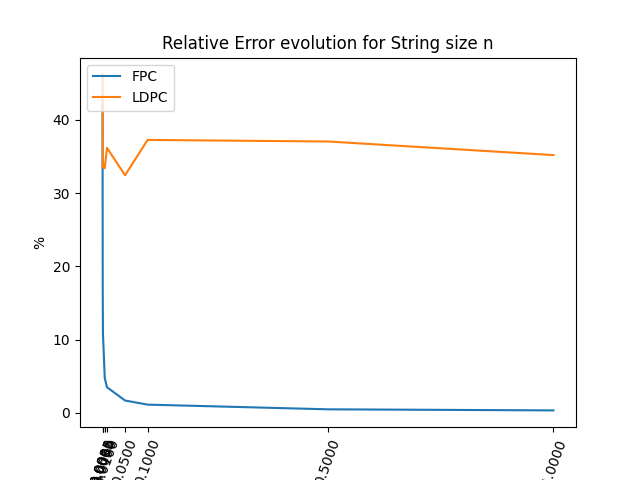
\includegraphics[scale=0.5]{relative_error_big.png}
\caption{Average relative error for chains size [100,500,1000,5000,10000,50000,100000,500000,1000000]}
\end{table}
Across all tests, $fpc$ outperforms $ldpc$ when it comes to relative error, mostly due to its consistent probability, which can cause big relative errors for smaller tests, but gets evened out for bigger tests as the random factor means less.\par
\begin{table}[H]
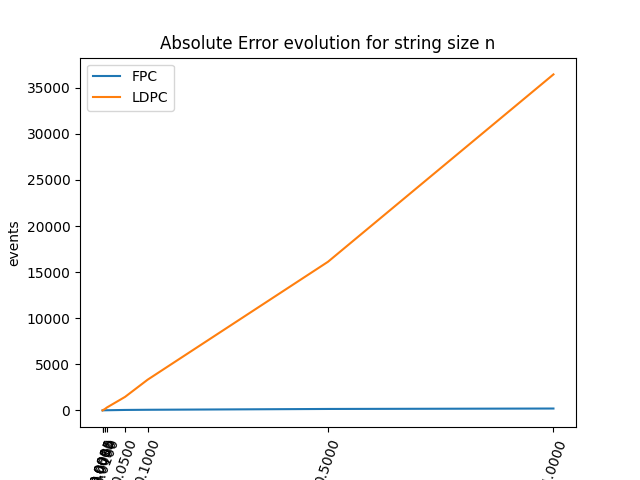
\includegraphics[scale=0.5]{absolute_error_big.png}
\caption{Average absolute error for chains size [100,500,1000,5000,10000,50000,100000,500000,1000000]}
\end{table}
As expected both methods have an increase in absolute errors, though $ldpc$'s is so big that it dwarfs $fpc$'s in comparison.\par
\begin{table}[H]
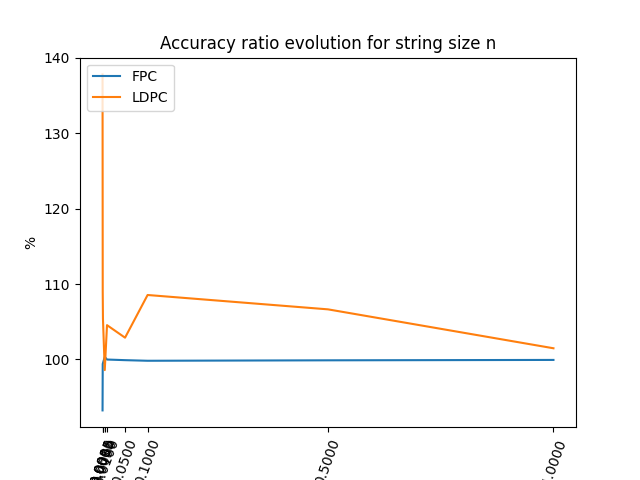
\includegraphics[scale=0.5]{accuracy_ratio_big.png}
\caption{Average accuracy ratio for chains size [100,500,1000,5000,10000,50000,100000,500000,1000000]}
\end{table}
Table III might be a bit misleading, it shows the $ldpc$'s average accuracy ratio leading to 100\%, but lots of big errors occur on both sides (100\%+ and 100\%-, which can be seen by its huge relative errors), making it average out on 100\%. The $fpc$'s value is much more reliable, as shown by its smaller relative errors.\par
\begin{table}[H]
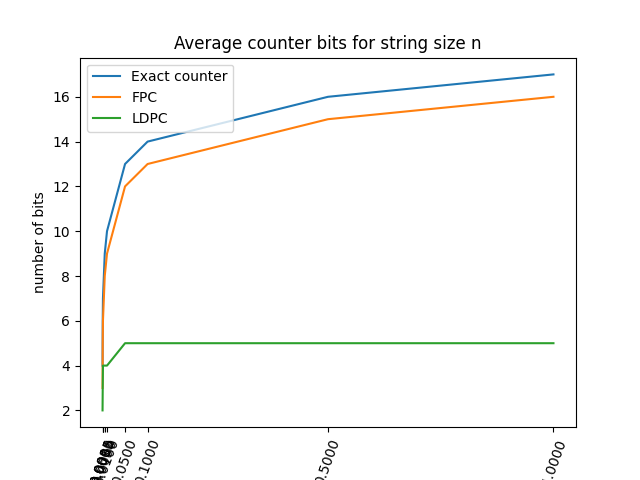
\includegraphics[scale=0.5]{average_counter_bits_big.png}
\caption{Average counter bits needed for chains size [100,500,1000,5000,10000,50000,100000,500000,1000000]}
\end{table}
As previously stated and also demonstrated on table IV, this is both the biggest advantage and disadvantage of the $ldpc$, as its small counters outperform both the $fpc$ and exact counters, but also lead to its imprecision, causing huge errors  as seen in  table I and II.\par

The most astounding difference above all else has to be the counter values of the $ldpc$, the counter of the most frequent character, $r$, increased from values around $8$ with test chain size $100$ to values surrounding the low $30$'s for chain size $1000000$. This is the main advantage of this approach. It may lose precision but it can keep its counters with extremely low values.
\section{Conclusions}
I think it's clear that both types of counters have their advantages and disadvantages, and I would be curious to see how they would perform for much bigger amounts of data though I am limited by my computer's processing power.
Regardless, it's a very interesting and demanding area, where progress is still needed. I'm interested in learning more about the subject and seeing what kinds of new approaches might come along in the following years.
%\section{References}


%[1]\url{https://en.wikipedia.org/wiki/Clique_(graph_theory)}
%[2]\url{https://en.wikipedia.org/wiki/NP-completeness}\par
%\
%[3]	A. Levitin, Introduction to the Design and Analysis of Algorithms, 3rd Ed., Pearson, Chapter 3,pp.97-98, 2012\par
%\
%[4]	A. Levitin, Introduction to the Design and Analysis of Algorithms, 3rd Ed., Pearson, Chapter 3,pp.115, 2012

\bibliography{bibliography}
\end{document}
